\documentclass{llncs}

\usepackage{hyperref}

\usepackage{pgf}

%\usepackage{amsmath,amssymb,amsfonts,amsthm,tikzcaption}
\usepackage{tikz}
\usetikzlibrary{arrows, decorations.pathmorphing, backgrounds, positioning, fit, petri, automata}

\usepackage[lined,boxed,commentsnumbered, ruled]{algorithm2e}


\usepackage{smartdiagram}

\begin{document}



\title{Questionnaire generation for better opinion polling}

\author{submitted for blind review}

\maketitle









\begin{abstract}

This paper studies a novel problem. Given a topic, how to automatically generate a polling questionnaire from a question bank collected from online debate forums? This is not a trivial task, as even opinion polls composed by human experts are not always reliable. We propose to model the problem as, on a bi-level topic sensitive question graph, selecting a minimal independent set that covers a maximal weighted set of key phrases. To construct the graph, we exploit both content information and estimated voting results. Quantative and qualitative experimental results demonstrate the competency of our methods.
\end{abstract}






\section{Introduction}\label{sec:intro}
%polling is important

Opinion poll is not uncommon in modern society. The first known example of an opinion poll was conducted nearly 200 years ago\footnote{\url{https://en.wikipedia.org/wiki/Opinion_poll}}. It successfully predicted the outcome of the United States presidency in 1824. Since then, it has been a convention to organize an opinion poll to measure public opinions and document the experiences. Nowadays, opinion polls cover a wide range of subjects, from market performance of a video game to presidential job approval ratings. Polling results provide valuable information for everyone on events in the news and other topics of interest, and facilitate in policy making and other decision makings.
%polling is a questionnaire

In an opinion poll, a series of questions are handed out to voters sampled from the target population. The goal of the poll is to extrapolate generalities based on the answers by sample voters. Thus the design of questionnaire is crucial. Conventionally polling questions are composed by professionals with expertise. There are polling organizations in virtually every country with elections. Major television networks also operate opinion pollings regularly. However, opinion polls are not always reliable in predicting public opinions on an unseen topic. For instance, Donald Trump's election in 2016 signals the biggest and complete poll failure ever.
%motivation

Recently, online social media site has become a dominant platform for online users to publish and exchange ideas and opinions. It has attracted researchers to study public opinions~\cite{OConnor2010tweets,Lampos2013user}. Online debate forums are in particular valuable for public opinion mining. In a debate forum, many simple agree/disagree scale questions are presented, and users are invited to vote and comment on one option. Some example questions and their comments are shown in Fig.~\ref{fig:example} .

%internet polling, problem definition(not formal)

From the view of opinion polling, a debate forum is a bank of polling questions. Is it possible to automatically generate an opinion poll for any given topic from online debate forums? In this paper, we explore the possibility of generating opinion polls more rapidly and less expensively. The following scenario is presented, given a crawl of online debate forums, the task is to automatically select appropriate polling questions from the crawl for any topic.

%problem
The task of question selection is far from trivial. There are some general guidelines to write questions in the community of pollsters. For example, it is well established that a poll should ask "enough questions to allow all aspects of an issue to be covered". The wording of each question should be carefully organized so that the true feelings of respondents are revealed~\footnote{\url{https://en.wikipedia.org/wiki/Opinion_poll}}. Keeping the questionnaire as short as possible is also a golden role~\cite{Trochim2000Research}. However, there is no known computational solution.

%framework

We propose a framework which is based on a \textbf{Bi}-level \textbf{T}opic \textbf{S}ensitive \textbf{Q}uestion \textbf{G}raph (BITSQG). The first layer of bi-level topic sensitive question graph represents the equivalences between questions, the second layer consists of key phrases weighted by how relevant they are to the given topic. To produce a polling questionnaire, we extract the minimal independent set of questions covering a maximal weighted set of key phrases.

%challenge

There are two challenges raised in the graph based framework. (1) How to match equivalent questions? Determining equivalent polling questions is beyond paring up semantically similar questions. Small changes of words in a question can lead to big changes in the answer. In the toy example in Fig.~\ref{fig:example}, it is difficult for teens to ``obtain'' marijuana, but it is easy for teens to ``buy'' marijuana\footnote{The toy example is a modified version of 2003 survey of teens and drug uses}.(2) How to extract key phrases and associate a topic relevance with each key phrase? On one hand, the questions are too short to provide enough co-occurrence information for any significance measure. On the other hand, questions are usually well formatted and the internal structure might be useful in detecting key phrases.

%contribution



Our contributions in this paper are three fold. (1) We study the problem of opinion poll generation for a given topic from a question bank collected from online debate forums. To the best of our knowledge, this is a novel problem. To tackle this problem, we present a framework which is based on a bi-level topic sensitive question graph. (2) We combine semantic similarity and response similarity to match equivalent questions. We utilize statistical inference technique and NLP strategies to detect distinguishing questions. (3) We employ sequential pattern mining techniques to extract and weigh key phrases. We conduct quantative and qualitative experiments on real data sets. Experimental results demonstrate that our proposed methods can generate high quality polling questionnaires.

%paper structure

This paper is structured as follows. We describe details of our framework and algorithms in Sec~\ref{sec:QG} and Sec~\ref{sec:BITSQG} . The experimental results are presented and analyzed in Sec~\ref{sec:experiment}. We briefly introduce related work in Sec~\ref{sec:relatedwork}. We give our introduction and an outlook for future work in Sec.~\ref{sec:conclusion}.

\begin{figure}[htbp]
\begin{center}
\begin{tabular}{|p{6cm}|p{6cm}|}
\hline
\multicolumn{2}{|l|}{$q_1$: Is it difficult for someone your age to buy marijuana?}\\
Pro: 390 & Con: 610 \\
Lexy: We still need doctor's documents& 
         Alice: A lot of drug selling occurs in my neighborhood\\
          ...& ...\\\hline
\multicolumn{2}{|l|}{$q_2$: Is it easy for someone your age to obtain marijuana?}\\
Pro: 150 & Con: 350 \\
Alice: In my experience, fairly simple & 
        Bob: Marijuana seeds are not everywhere\\
          ...& ...\\\hline
\multicolumn{2}{|l|}{$q_3$:  Is it easy for someone your age to find marijuana?}\\
Pro: 630 & Con: 270 \\
 Shania: Most of my friends used marijuana, if not all & 
        Coco: Not in medical marijuana clinics \\
          ...& ...\\\hline
\multicolumn{2}{|l|}{$q_4$: Should governments legalize marijuana?}\\
Pro: 590 & Con: 210 \\
Fanny: It should be legalized, regulated, and taxed. &
Anon:No it makes people lazy and unproductive. Driving while high is a serious problem.\\
...& ...\\\hline

\multicolumn{2}{|l|}{$q_5$: Should marijuana be illegal?}\\
Pro: 185 & Con: 420 \\
Tygaa: Marijuana makes you have a slow reaction to every thing. This drug makes you have car crashes.&
Arget: It should be taxed and regulated. Marijuana is less harmful than tobacco and alcohol.\\
...& ...\\\hline

  \end{tabular}
\caption{An illustrative example of opinion poll generation}
\label{fig:example}
\end{center}
\end{figure}


\section{Question Graph}\label{sec:QG}

The problem setup is based on online debate forums. An online debate forum is a set of questions $Q=\{q\}$, Each question is a tuple $q=(T_q,N_q,P_q)$, where $T_q$ is the question's textual content. We only deal with dual-sided debates, thus $P_q$ is the pro-stance, and $N_q$ is the con-stances. In online debate forums, users argue why their viewpoint is right by commenting on the chosen vote option. We model $N_q,P_q$ as a set of vote-comment pairs $<\vec{u},c>$, where $\vec{u}$ is the user portfolio vector, and $c$ is the comment's textual content. We adopt the bag-of-word representation for all text segments $T_q,c$.



To enable the application of graph-based opinion poll generation, we first introduce the concept of question graph. A question graph is an undirected graph $G=(Q,E)$ formed by a set of nodes and a set of edges. Without ambiguity, we use the same symbol $q$ to denote both questions and nodes in the question graph. Each edge $e(q,q')\in E, q,q'\in Q$ connecting $q$ and $q'$ indicates that the corresponding questions $q,q'$ are interchangeable. For the cause of opinion polling, we make the hypothesis that, two questions $q,q'$ are interchangeable if (1) they are semantically similar (2) they yield similar polling results. Therefore we first present a clustering algorithm to construct cliques of semantically similar questions, and then we break ties between questions that result in distinguishing estimated voting responses.



\subsection{Semantic Clustering}\label{sec:clustering}



As we can not specify the number of semantic clusters, we need a non-parametric clustering algorithm. For this purpose, we use the \textbf{A}ffinity \textbf{P}ropagation (AP) algorithm. The idea of AP is to identify exemplars and assign remaining data points to nearest exemplars. The algorithm stores information in two matrices: $R,A$. The ``responsibility'' matrix $R=\{r(i, j)\}$ measures how well a data point $j$ can represent $i$. The ``availability'' matrix $A=\{a(i,j)\}$ quantifies how appropriate it is for $i$ to pick $j$ as an exemplar.



The AP algorithm starts by initializing both matrices to all zeroes, and proceeds to update $R,A$ iteratively. $R$ is updated by passing messages from cluster members to cluster exemplars. $A$ is updated by passing messages from cluster exemplars to cluster members.

\begin{eqnarray}
r(i,j)\leftarrow s(i,j)-\max _{j'\neq j}\{a(i,j')+s(i,j')\}\\
a(i,j) \leftarrow \min \{ 0, r(j,j) + \Sigma_{i' \not\in \{i,j\}} \max(0, r(i',j)) \} \\
a(i,i) \leftarrow \sum_{i' \neq i} \max(0, r(i',i))
\end{eqnarray}


The updating messages are based on similarity function $s(i,j)$. It is worth noted that affinity propagation doesn't require the similarities to be symmetric, as long as the similarity function satisfies the following properties.



\textbf{Property 1} $s(i, j) > s(i, j')$ if and only if $i$ is more similar to $j$ than to $j'$.



Since the similarity function plays an important role in AP, we tailor a similarity measurement for question clustering. Intuitively, key phrases are most significant featurs of questions. We use $SF(q)=\{k,k \in T_q\}$ to denote the key phrases contained in question $q$. The extraction of key phrases will be introduced in Sec.~\ref{sec:BITSQG}. The similarity function is defined as:



\begin{equation}\label{equ:similarity}
s(i,j)=\frac{|SF(i)\bigcap SF(j)|}{|T_i|}
\end{equation}





According to Equ.~\ref{equ:similarity}, if the two questions have more common key phrases, then they are more similar. The dominator is only related to question $i$. If two pairs $<i,j>$ and $<i,j'>$ have the same number of common key phrases, then the similarities $s(i,j)=s(i,j')$. This ensures that the length of questions as cluster members will not affect the ``responsibility'' and ``availability'' of the exemplars.





The AP algorithm stops when the cluster boundaries stay unchanged or the maximal number of iterations is achieved. The nodes with positive self similarities are chosen as exemplars. %The algorithm is shown in Algorithm~\ref{algo:AP}



%\begin{algorithm}[!t]
%\caption{AP algorithm for question clustering\label{algo:AP}}
%\KwIn{ $R=A=\bf{0}$, maximal number of iterations $N$, key phrases $\{SF(q),q\in Q\}$ and textual contents $\{T_q,q \in Q\}$}
%\KwOut{$C$}
%\For{$n=0;n<N;n++$}
%{
%\For{$i,j \in Q$}
%{
%$s(i,j)=\frac{|SF(i)\bigcap SF(j)|}{|T_i|}$\;
%$r(i,j)\leftarrow s(i,j)-\max _{j'\neq j}\{a(i,j')+s(i,j')\}$\;
%}
%\For{$i,j \in Q, i\neq j$}
%{
%$a(i,j) \leftarrow \min \{ 0, r(j,j) + \Sigma_{i' \not\in \{i,j\}} \max(0, r(i',j)) \} $\;
%}
%\For{$i \in Q$}
%{
%$a(i,i) \leftarrow \sum_{i' \neq i} \max(0, r(i',i))$\;
%\If{$ (r(i,i)+a(i,i))>0$}
%{$c_i=i$\;}
%}
%\For{$i \in Q, c_i \neq i$}
%{
%$c_i=\arg \max_{j \neq i} (r(i,j)+a(i,j))$
%}
%}
%Return $C$\;
%\end{algorithm}

\subsection{Questions with Distinguishing Responses}\label{sec:pair}
We have shown in Sec.~\ref{sec:intro} that, even slight wording differences between semantically similar questions can lead to distinguishing responses. To generate an accurate polling questionnaire, it would be ideal to measure question similarities in the sense of wording quality. However, the effects of wording are too complicated to derive a simple similarity metric. We present to detect questions with dissimilar wording choices by directly using the responses. 

In online debate forums, each question is voted and commented by a group of users. For simplicity, we presume that this group of users gets together randomly. The question-answering process is equivalent to conducting a polling with one question. In statistics, the margin of error is used to interpret the polling result. For a question $q$, the ratio of people holding a pro-stance is $\sigma(q)=|P_q|/(|P_q \bigcup N_q|)$, the margin of error is $MOE(q)=\frac{1}{\sqrt{ n(q)}}\times 100\%$, where $n(q)=|P_q\bigcup N_q|$ is the number of votes (and comments) for question $q$, then the estimated response interval will be:

\begin{equation}
I(q)=[\sigma(q)-MOE(q),\sigma(q)+MOE(q)]
\end{equation}



For example,  $1000$ people answer question $q_1$ in Fig.~\ref{fig:example}, $61\%$ of them think that buying marijuana is easy. Based on this sample, we are $95\%$ confident that between $58\%$ and $64\%$ of all users on the debate forum think that buying marijuana is easy.  $500$ people answer question $q_2$, $30\%$ of them consider obtaining marijuana is easy. We can predict  that the percentage of people who agree that obtaining marijuana is easy will be in the range of $[25.5\%,34.5\%]$ with $95\%$ confidence.

Intuitively, if two questions are both worded nicely to reflect the true public opinion, then the resulting output must accord with each other. If the two questions have non-overlapping response ranges, then the wordings must be distinguishing.  Based on this hypothesis, we present the following steps.

After semantic clustering in Sec~\ref{sec:clustering}, we construct cliques of queries, where every pair of queries are connected. Then we remove edge $e(q,q')$ between questions who have non-overlapping response intervals $I(q)\bigcap I(q')=\emptyset$. For example, for the questions in Fig.~\ref{fig:example}, we first construct two cliques, then we remove the edges $(q_1,q_2),(q_2,q_3)$. The steps are shown in Fig.~\ref{fig:steps}.

\begin{figure}
\begin{minipage}[b]{.2\textwidth}
\centerline{
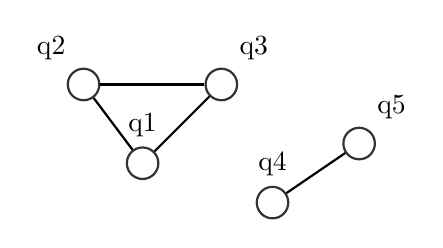
\begin{tikzpicture}[scale=0.5]
\tikzstyle{q}=[circle, minimum size = 4mm, thick, draw =black!80, node distance = 10mm]
\tikzstyle{connect}=[-, thick]
\node[q,label=120:{ q2}] (v2) at (-3, 0) {};
\node[q,label=90:{ q1}] (v1) at (-1.5, -2) {};
\node[q,label=60:{ q3}] (v3) at (0.5, 0) {};
\node[q,label=90:{ q4}] (v4) at (1.8, -3) {};
\node[q,label=60:{ q5}] (v5) at (4, -1.5) {};
\path (v2) edge [connect] (v1);
\path (v2) edge [connect] (v3);
\path (v1) edge [connect] (v3);
\path (v4) edge [connect] (v5);
\end{tikzpicture}
}
\centerline{Step 1: semantic clustering}
\end{minipage}
\hfill
\hspace{-100pt}
\begin{minipage}[b]{.2\textwidth}
\centerline{
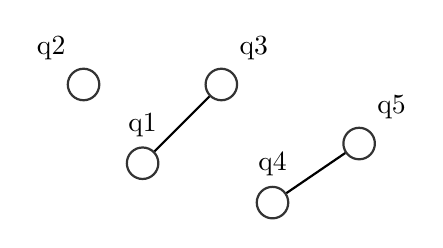
\begin{tikzpicture}[scale=0.5]
\tikzstyle{q}=[circle, minimum size = 4mm, thick, draw =black!80, node distance = 10mm]
\tikzstyle{connect}=[-, thick]
\node[q,label=120:{ q2}] (v2) at (-3, 0) {};
\node[q,label=90:{ q1}] (v1) at (-1.5, -2) {};
\node[q,label=60:{ q3}] (v3) at (0.5, 0) {};
\node[q,label=90:{ q4}] (v4) at (1.8, -3) {};
\node[q,label=60:{ q5}] (v5) at (4, -1.5) {};
\path (v3) edge [connect] (v1);
\path (v4) edge [connect] (v5);
\end{tikzpicture}}
\centerline{Step 2: remove edges}
\end{minipage}
\caption{Construct a question graph in the toy example}
\label{fig:steps}
\end{figure}

We measure the response similarity based on estimated portion of pro-stances. There is one more issue left: how to match the pro-stances between a pair of similar questions?  The pro-stances for each question do not always refer to the same opinion. For example, the pro-stance of question $q_1$ is actually mapped to the con-stance of question $q_2$ in Fig.~\ref{fig:example}. 

We treat the pro-stance matching task as a binary classification task. Suppose we are given two questions $q,q'$, we train a classifier so that the output is positive if $P_q$ matches to $P_{q'}$ while output is negative if $P_q$ matches to $N_{q'}$.  We use features from 4 fields: text, vote, demographic and sentiment. From each field, we derive two features indicating how much the output will be positive and negative respectively. 

As shown in the toy example, the stance can be recognized from the comments. For example, the pro-stance of $q_3$ and the con-stance of $q_4$ are much alike in vocabulary. The text field is the combined textual body of the question and all of its comments. Intuitively, two stances are identical if their text fields are similar. We use cosine similarity to compare two stances. $f_1$ is a feature correlated to positive output, $f_2$ is correlated to negative output.

\begin{eqnarray}
f_1= cosine (P_q,P_{q'})+cosine (N_q,N_{q'}) \\
f_2= cosine (P_q,N_{q'})+cosine (N_q,P_{q'})
\end{eqnarray}


The stance can also be identified if a user votes for both questions. Hypothetically, a user will stick to one stance. For example, in the toy example, Alice votes for both $q_1,q_2$, and the con-stance in $q_1$ is the pro-stance in $q_2$. For a pair of instances, the more common voters they have, the more likely the two stances will be matched.

\begin{eqnarray}
f_3=|\{u|u\in P_q,u\in P_{q'}\}|+|\{u|u\in N_q,u\in N_{q'}\}| \\
f_4=|\{u|u\in P_q,u\in N_{q'}\}|+|\{u|u\in N_q,u\in P_{q'}\}|
\end{eqnarray}


We further extend the hypothesis on an individual vote to group votes. We believe that for a group of users with similar demographic attributes, the opinion distribution will be stable. We consider groups determined by party (demographic and republicans) and age ( $20-,20-40,40+$). For each group $g$ on question $q$, we compute the pro-stance frequency $ps(q,g)=[|\{u|u\in g, u \in P_q\}|$ and the con-stance frequency $cs(q,g) =|\{u|u\in g, u \in N_q\}|]$. We summate cosine similarities between stance frequency vectors over all groups. 

\begin{eqnarray}
f_5= \Sigma_g cosine([ps(q,g),cs(q,g)],[ps(q',g),cs(q',g)]) \\
f_6=\Sigma_g cosine([ps(q,g),cs(q,g)],[cs(q',g),ps(q',g)])
\end{eqnarray}


We exploit the sentiments in the query to match stances.  We extract negative opinion words by the FBS lexicon~\cite{Hu2004Mining}. Suppose $n(q)$ is the number of negative opinion words in question $q$, since a double negative turns the opinion to a positive, we have:  

\begin{eqnarray}
f_7=1-[n(q)-n(q')]\%2\\
f_8=[n(q)-n(q')]\%2
\end{eqnarray}




\section{Questionnaire Generation}\label{sec:BITSQG}

\subsection{Bi-level Topic Sensitive Question Graph}

The question graph constructed in Sec.~\ref{sec:QG} is static. To generate the polling questionnaire for a given topic, we first need to build a dynamic graph induced by the topic.  A BITSQG induced by topic $o$ consists of two layers  $BITSQG^o=(Q,E,K,W^o,A)$. The first layer is the question graph, the second layer is a set $K$ of key phrases, where each node is assigned a weight $w^o(k),k\in K$. The two layers are connected by arcs in $A$. An arc $a(q,k)$ is added to the BITSQG if the question $q$ (either in the question body or in one of the comments) contains key phrase $k$. An illustrative BITSQG is shown in Fig.~\ref{fig:BITSQG}

We extract key phrases in questions as the basic semantic units. Conventionally, key phrase extraction is implemented by filtering out statistical significant phrases. However, the questions are too short and sparse and do not offer enough statistics. We observe that questions in online debate forums are well formatted. For example, many questions are in the form ``should ... be ...?'' We employ sequential pattern mining algorithm to detect common question templates. 

For a question which satisfies several templates, we remove the longest template. The remaining part is considered to be a key phrase. For example, question ``Should capital punishment be legal ?'' satisfies two templates  ``should...be...'' and `` should... be legal''. We delete the longest template from the question and obtain ``capital punishment''.

The weights of key phrases in BITSQG indicate the relevance of key phrases to the topic. The relevance depends on co-occurrence in both question and comments. The relevance $w^o(k)$ of each key phrase $k$ to a given topic $o$ is defined by

\begin{equation}
w^o(k) = w_1\times | Q(o)\bigcap Q(k)| + w_2 \times (| Q(o)\bigcap C(k)| + | Q(k)\bigcap C(o)|)
\end{equation}

where $Q(o)$ is the set of queries containing the key phrase $o$ in the query texts, $C(k)$ is the set of queries containing the key phrase $k$ in the comments, $w_1,w_2$ are coefficients.


\begin{figure}
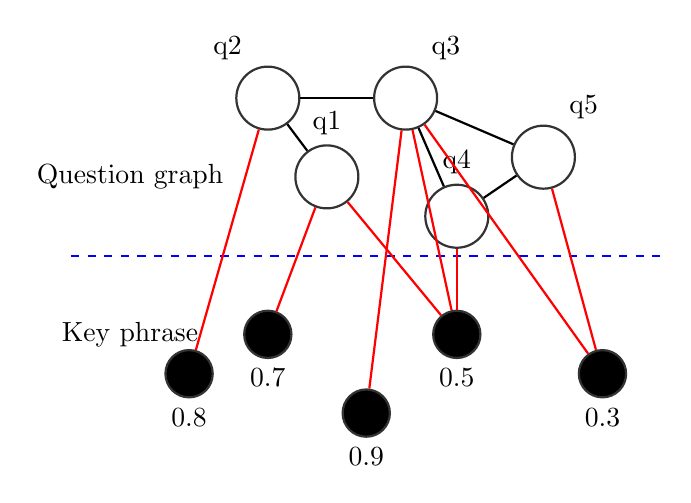
\begin{tikzpicture}[scale=0.5]
\tikzstyle{q}=[circle, minimum size = 8mm, thick, draw =black!80, node distance = 10mm]
\tikzstyle{key}=[circle, fill=black, minimum size = 6mm, thick, draw =black!80, node distance = 10mm]
\tikzstyle{connect}=[-, thick]
\node (qtitle) at (-6.5, -2) { Question graph};
\node[q,label=120:{ q2}] (v2) at (-3, 0) {};
\node[q,label=90:{ q1}] (v1) at (-1.5, -2) {};
\node[q,label=60:{ q3}] (v3) at (0.5, 0) {};
\node[q,label=90:{ q4}] (v4) at (1.8, -3) {};
\node[q,label=60:{ q5}] (v5) at (4, -1.5) {};
\node (ktitle) at (-6.5, -6) {Key phrase};
\node[key,label=below:{ 0.8}] (k1) at (-5, -7) {};
\node[key,label=below:{ 0.7}] (k2) at (-3, -6) {};
\node[key,label=below:{ 0.9}] (k3) at (-0.5, -8) {};
\node[key,label=below:{ 0.5}] (k4) at (1.8, -6) {};
\node[key,label=below:{ 0.3}] (k5) at (5.5, -7) {};
\path (v2) edge [connect] (v1);
\path (v2) edge [connect] (v3);
\path (v3) edge [connect] (v4);
\path (v3) edge [connect] (v5);
\path (v4) edge [connect] (v5);
\draw[blue,dashed] (-8,-4) edge [connect] (7,-4);
\path[red] (v2) edge [connect] (k1);
\path[red] (v1) edge [connect] (k2);
\path[red] (v1) edge [connect] (k4);
\path[red] (v3) edge [connect] (k3);
\path[red] (v3) edge [connect] (k4);
\path[red] (v3) edge [connect] (k5);
\path[red] (v4) edge [connect] (k4);
\path[red] (v5) edge [connect] (k5);
);
\end{tikzpicture}
\caption{An illustration of BITSQG}\label{fig:BITSQG}
\end{figure}

\subsection{Minimal Independent Questions Covering Maximal Key Phrases}

The questionnaire needs to be concise, while preserving the coverage of relevant key phrases. In BITSQG, two questions are connected if they are semantically similar and they produce similar polling responses. This means that if we have two adjacent questions in the result, the questionnaire will be redundant.  In other words, our target is an independent question set. An independent question set $S\subset Q$ is a set of questions where no two nodes are adjacent.   


For an arbitrary set $S\subset Q$ of questions, the sum of weights of key phrases it covers on topic $o$ is  defined as 
\begin{equation}
w^o(S)=\Sigma_{q\in S, a(q,k)} w(k)^o 
\end{equation}

To generate the questionnaire, we aim to select a \textbf{M}inimal \textbf{I}ndependent set covering a \textbf{M}aximal \textbf{W}eighted set of key phrases (MIMW).  $S$ is a MIMW if and only if (1) S is an independent question set; (2) there is no independent set $S'$ that  $W^o(S')>W^o(S)$; (3) there is no independent set $S'$ with $W^o(S')=W^o(S)$ that $|S'|>|S|$.  For example?in Fig.~\ref{fig:BITSQG}, the MIMW set is $\{q_2,q_3\}$. 

The MIMW problem is NP-hard given that the independent set problem is known to be NP-hard. A greedy algorithm can achieve approximate rate of $1 + \log(\Delta\|OPT\|)$, where $\Delta$ is the maximal degree of $BITSQG$ and $OPT$ is the optimal set. We present the greedy algorithm to select a subset of questions. Starting from an empty set, at each step, we select the question whose covering weight is maximum. 

 \begin{algorithm}[htbp]\label{alg:MIMW}
\caption{Greedy $MIMW$ Approximation}
\KwIn{$BITSQG=(Q,E,K,W^o,A)$}
\KwOut{MIMW set $S$}
$S\leftarrow\emptyset$\;
\While{$|K|\neq \emptyset$}
{

\For{$q\in Q$}
{
$w(q)=\Sigma_{k\in K, a(q,k)} w(k)^o$\;
}
$q\ast=\arg\max_{q \in Q} w(q)$\;
$S \leftarrow S \bigcup \{q\ast\}$\;
$Q \leftarrow Q-\{q\ast\}$\;
$K \leftarrow K -\{k|a(q\ast,k) \in A\}$\;
}
\end{algorithm}

\section{Experimental Analysis}\label{sec:experiment}

\subsection{Experimental Setup}

The data set used in the experiment is obtained from a large online debate forum\footnote{http://www.debate.org/opinions/politics}. We crawl $14,620$ questions published before February 2nd, 2017 on the largest topic: politics. For each question, we crawl all the votes and comments ($152946$ votes), We crawl the user profiles for each user participating in at least one question. The user demographics include party, ethnicity, age group and other 22 attributes.  

In pre-processing, we remove anonymous users and questions without comments, reduce the number of questions to $6777$ and the number of comments to $28,911$. We remove english stop-words and run Porter Stemmer. Stop-word removal and stemming significantly decrease the length of questions and comments. The default weighing scheme is tf-idf. The statistics are shown in Tab~\ref{tab:data}. 


\begin{table}[htp]
\caption{Statistics of data set}
\begin{center}
\begin{tabular}{|c|c|c|c|c|c|}
\hline
Number of questions  & 6777 & Avg. length  before & 12.22 & Avg. length  after & 5.66\\\hline
Number of comments & 28911 & Avg. length  before & 118.51 & Avg. length  after & 55.94\\\hline
Number of users &16739 & Avg. votes per user & 1.73 & - & -\\\hline
\end{tabular}
\end{center}
\label{tab:data}
\end{table}%



\subsection{Matching Questions}

In constructing the BITSQG, one important step is to match questions. This involves semantical clustering (described in Sec.~\ref{sec:clustering}) and pairing up voting options (described in Sec.~\ref{sec:pair}).  

To evaluate the performance of matching questions, we use a ground truth which includes equivalent questions and correct matching of stances. The ground truth is manually labeled. 300 questions are randomly selected  from all questions. Two students are invited to first manually label semantically equivalent questions, then map the stances between equivalent questions. A total of 1437 question pairs are produced,  945 pairs are with the same polarities, i.e. a pro-stance is mapped to a pro-stance of another question, or a con-stance is mapped to a con-stance; and  492 pairs are with opposite polarities, i.e. a pro-stance is mapped to a con-stance.

The evaluation metric is precision, which is the ratio of correctly recognized stance pairs. 
\begin{equation}
Precision = \frac{|R\bigcap T|}{|R|}
\end{equation}
where $R$ is the set of pairs recognized, $T$ is the set of pairs in the ground truth.

We conduct the modified AP algorithm on all questions and comments. Parameter $damping=0.5$, maximal number of iteration is set to be $N=200$. For questions without comments, when $preference=median(S)$ we obtain 783\footnote{The number of clusters is based on the entire data set, not just the ground truth.} clusters, when $preference=2*median(S)$ we obtain 335 clusters. For questions with comments, we obtain 527,204,121 clusters when $preference=median(S),2*median(S),3*median(S)$. We compare AP with a parametric clustering algorithm: K-means. The comparative methods for pairing up stances include: (1) Default: which is to pair a pro-stance of a question to a pro-stance of a similar question; (2) Text: the proposed classification algorithm based on textual features $f_1,f_2$; (3) Vote: classification based on votes $f_3,f_4$; (4) Demographic: classification based on groups of votes $f_5,f_6$ (5) Sentiment: classification based on sentimental features $f_7,f_8$ (6) Combine: classification based on all 8 features.

\begin{figure}[htbp]
\begin{center}
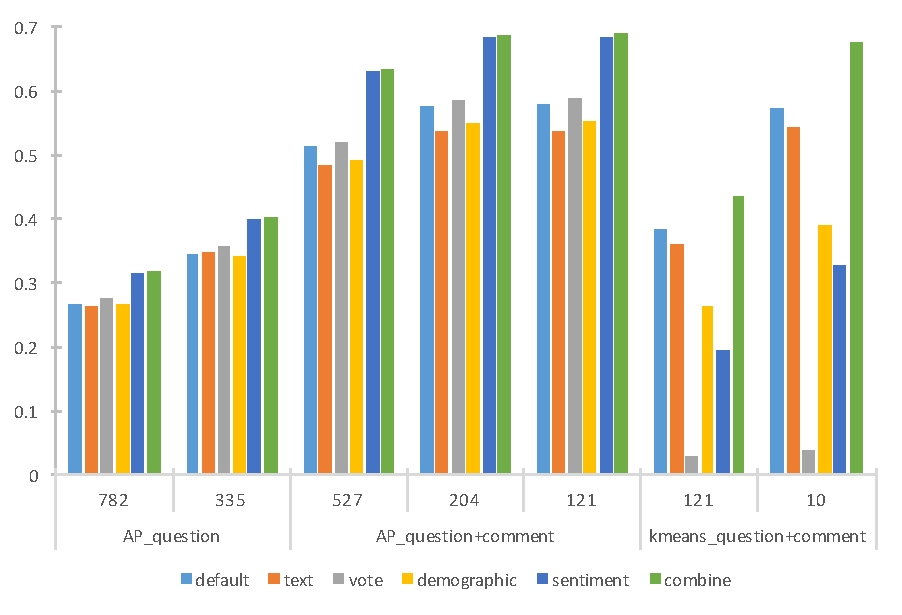
\includegraphics[scale=0.5]{match.pdf}
\caption{Precision of various features and clustering methods for paring up stances of questions}
\label{fig:performancepair}
\end{center}
\end{figure}

We have the following observations from Fig.~\ref{fig:performancepair}. (1) Textual content in comments provide valuable information.  AP on questions and comments is superior (almost doubles) than AP on questions only for various settings. (2) AP can determine the best number of clusters. The performance of AP with 204 clusters is very similar to that with 121 clusters.  The best performance of AP with 121 clusters on combined features is $0.6896$, when there are 121 clusters, the precision is $0.6875$. This shows that AP converges to the best number of clusters. (3) When the number of clusters for K-means is set to be the number of clusters obtained by AP, the performance is dramatically reduced by $40\%$. This again verifies that AP has the ability to self-adjusting to the optimal clustering. (4) When we set the number of clusters to be $10$, the performance of Kmeans increases by roughly $40\%$. It suggests that the K-means needs a smaller number of clusters. However the performance is still slightly worse than the performance of AP with 204 and 121 clusters.The underlying problem is that the questions are about a wide range of topics, in nature they are very dissimilar. A large number of clusters is more reasonable. (5) Combining various features always achieves the best precision. For AP methods, sentimental features alone can produce comparative performance, while for K-means methods, it is more important to combine all features than to depend on a single type of features.   

\subsection{Key Phrase Extraction and Weighing}

We next evaluate the performance of key phrase extraction and weighing. We use Prefixspan~\cite{Han2001Prefixspan} to discover question templates. We set the minimum support to $min\_support = 10$.  The top discovered question templates are .

\begin{itemize}
\item  should/can ... be/to/in/of ... ?
\item  do you agree/think/believe/support that ... is ... ?
\item is it/this/that ... ?
\item ... yes or no?
\end{itemize}



To evaluate the performance of key phrase weighing, we select e topics $o=$``gay marriage,gun control, drug abuse'', then from the extracted key phrases, we manually score the key phrase in a scale of $1-5$. In this manner, we obtain a ranking list of key phrases. We also rank key phrases based on the weights given by Sec.~\ref{sec:BITSQG}. 

The evaluation metric is NDCG, which is a standard measure for ranking systems.   $NDCG=\Sigma_L NDCG@L$, where $NDCG@L$ is the normalized discounted cumulative gain for top $L$ results. 

\begin{equation}
NDCG@L=\sum\limits_{i=1}^{M}\frac{\sum_{l=1}^{L}(2^{r_{i}(p(l,i))}-1)/log(1+l)}{M\sum_{l=1}^{L}(2^{r_{i}(t(l,i))}-1)/log(1+l)}
\end{equation}
where $p(l,i)$ is the index of the key phrase sorted in descending order by $w(k)^o$, $t(l,i)$ is the index of the key phrase sorted in descending order by human judges.

To demonstrate the performance of different coefficients $w_1,w_2$, we set  $w_1=100, w_2=w_1/x$. The NDCG with varying $x$ is shown in Fig.~\ref{fig:performancepair}. We can see that: (1) The key phrase weighing scheme performs good as NDCGs for all $x$ are high, approximately 1. (2) The best performance in term of NDCG is achieved when $x=5,NDCG=0.9865$. (3) The sharp decrease of NDCG when $x>5$ indicates that though comments are not as important as questions, their importance should not be ignored.

\begin{figure}[htbp]
\begin{center}
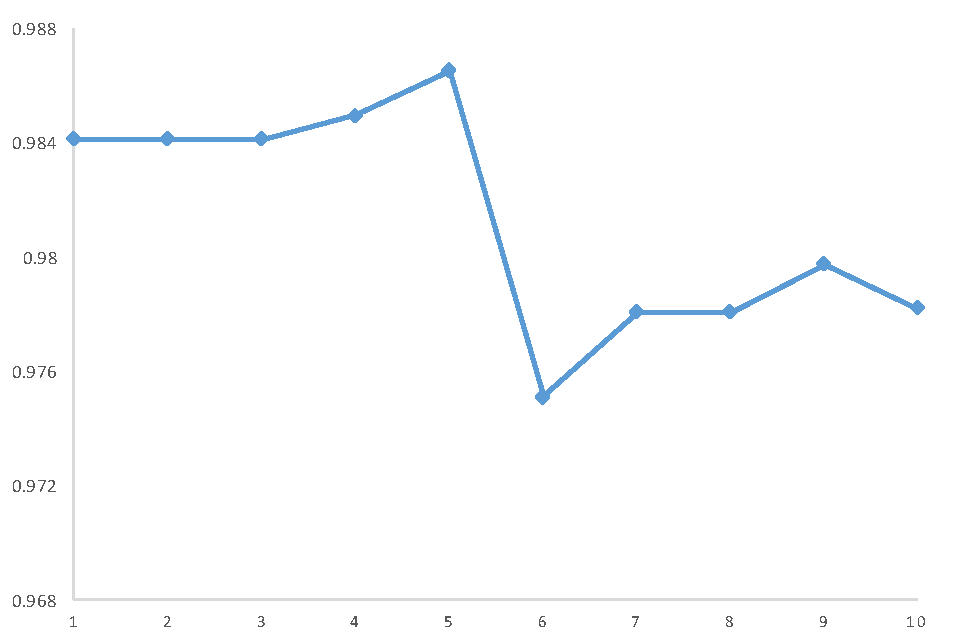
\includegraphics[scale=0.3]{NDCG.pdf}
\caption{NDCG of key phrase ranking on different values of $x$, $w_1=100, w_2=w_1/x$}
\label{fig:performancepair}
\end{center}
\end{figure}

\subsection{Evaluating the wording quality}
We conduct a qualitative study of the questionnaire generated.  According to the general guidelines for writing polling questions in~\cite{Trochim2000Research}, we conduct a user survey. The subjects of the survey are w students. Each participant is asked to read the questionnaires for 4 topics generated by different systems, without knowing which system generates which questionnaire. The participants must compare the results of different systems in a random order from the following point of views:  (1) Coverage: does the questionnaire cover all relevant issues? (2) Diversity: are the questions diversified, e.g. each question is about one issue at a time? (3) Simpleness: does the question use simple language and is it more easily understood by respondents? (4)Concreteness: is the question clear and specific and that each respondent will be able to answer? (5)Offensiveness: are there certain words that may be viewed as offensive to some respondents? (6) Emotion: are there words that may provoke emotional reaction? A score of 1 to 5 needs to be assigned to each system according to the user's satisfaction of the results. For coverage, diversity, simpleness and concreteness, a rank of 5  indicates that the result of the system is the most satisfactory. For the rest two aspect, a rank of 1 indicates the best system. 


As the questionnaire generation resembles the task of summarizing most informative questions, we compare our system to various summarization systems. The comparative methods are (1) Random: questions are randomly selected. (2) Sumbasic: this algorithm greedily selects the set of questions covering the maximal weights of key phrases. (3) TextRank~\cite{Mihalcea2004TextRank}: a graph-based ranking model for text summarization. (4) LexRank~\cite{Erkan2004LexRank}: a graph-based ranking model which selects sentences with most lexical centrality. (5) LSA ~\cite{Gong2001Generic}: a text summarization framework which uses the latent semantic analysis technique to identify semantically important sentences.
\begin{table}[htp]
\caption{User Study of Different Questionnaire Generation Systems}
\begin{center}
\begin{tabular}{|c|c|c|c|c|c|c|}
\hline
& coverage & diversity & simpleness & concreteness & offensiveness & emotion \\\hline
random & 2.25 & 4.875 & 3.125 & 2.5 & 1.25 & 1.625 \\\hline
sumbasic & 3.25 & 4.5 & 4.25 & 2.125 & \textbf{0.625} & \textbf{0.625} \\\hline
TextRank & 2.875 & 5 & 3.5 & 3.375 & 1 & 0.875 \\\hline
LexRank & 3.125 & 5 & 4.125 & 3.125 & 1.25 & 2.125 \\\hline
LSA & 2.5 & 5 & 2.125 & 3.125 & 1.125 & 1.875 \\\hline
MIMW & \textbf{3.5} & \textbf{4.875} & \textbf{4.25} & \textbf{3.75} & 0.75 & 0.75 \\\hline
\end{tabular}
\end{center}
\label{tab:userstudy}
\end{table}%

As shown in Tab.~\ref{tab:userstudy}, our system achieves best performance in coverage, diversity, simpleness and concreteness. Our system is the second best in terms of offensiveness and emotion. The user study demonstrate that the questionnaire produced by our system satisfies the general requirements for opinion polling composition.


Finally we present a case studies. The  topic is ``drug abuse''. As shown in Tab.~\ref{tab:casestudy}, each system selects 3 questions. The questions selected by our model are simple, clear, concrete, unbiased, and easily understood. Each covers a different aspect of the topic. On the contrary, some questions selected by other systems are confusing, i.e. asking ``is it OK ..'' can be misleading. Some systems tend to choose long questions, i.e. Random and LSA. It could be harmful for estimating the best polling results.
\begin{table}[htp]
\caption{Case study: questionnaire on ``drug abuse''}
\begin{center}
\small
\begin{tabular}{|p{2cm}|p{13cm}|}
\hline
Random &
 -Millionaire invests in marijuana start-up company: Should marijuana become a mainstream product and be marketed as such?
 
-Is it ok for the government to legalize drugs?
 
-Should employers be allowed to subject employees to mandatory drug testing?
\\\hline

SumBasic
&
- Should the U.S. legalize marijuana?

- Should drugs be illegal?

- Should welfare recipients be drug tested?
\\\hline

TextRank &

- Should the recreational use of marijuana be made legal in the United States?

- Should the House consider the war on drugs to be an effective policy among free people?

- Should welfare recipients be drug tested?
\\\hline

LexRank
&

- Is there a good reason why marijuana is illegal and alcohol and tobacco are legal?

- Should drugs be illegal?

- Is it ethical to drug test welfare recipients?
\\\hline

LSA
&

- Should individual states have more or less power compared to the federal government when implementing laws dealing with legalization of marijuana gay marriage and abortion?

- Has the War on Drugs really resulted in 45 million Americans being locked up for drug-related offenses at a cost of trillions?

- If welfare recipients are drug tested should we also test them for alcohol
\\\hline

MIMW
&

- Should the recreational use of marijuana be made legal in the United States?

- Should all drugs be legalized?

- Should someone receiving welfare be drug tested?
\\\hline

\end{tabular}
\end{center}
\label{tab:casestudy}
\end{table}%


\section{Related Work}\label{sec:relatedwork}
More and more work are devoted to mining and analyzing publicly available opinionated texts. The first line of work is to extract opinions, i.e. classifying positions and stances~\cite{Murakami2010Support}. The second line is to summarize public opinions, i.e. generating an opinion summary~\cite{Potthast2010Opinion}, or visualizing the polarity of each aspect of a product~\cite{Meng2012Entitycentric,Moghaddam2013FLDA}. Some works study the problem of opinion leader identification~\cite{song2007identifying} , or opinion search~\cite{Gerani2010Proximity}. Some recent works attempt to link text sentiment on online social media sites to polling results ~\cite{OConnor2010tweets,Lampos2013user}. However, polling is still essential if we prefer a more accurate and detailed opinion survey. This is a relatively unexplored area in the opinion mining literature.


The work in this paper is also related to research areas of text summarization. In particular, the polling questionnaire is similar to extractive summarization, where a concise set of units must be selected from a bunch of candidates. Many extractive summarization models are graph based~\cite{Mihalcea2004TextRank,Erkan2004LexRank,Gong2001Generic}. They follow a general procedure, where they first construct of graph of textual units (i.e. sentences or minimal meaningful units), then they compute salience for each textual unit on the graph. Our proposed framework is inspired by previous summarization methodologies.





\section{Conclusion}\label{sec:conclusion}
In this paper we study a novel problem of questionnaire generation. We propose a framework which is based on a bi-level topic sensitive question graph. We combine semantic similarity and similarities in responses to match equivalent questions. We conduct comprehensive quantative and qualitative experiments to verify the competency of our methods. 

One possible limitation of the proposed work is that we assume that the users randomly pick a question to vote. This may be an idealized situation. Selection bias occurs when the samples are not randomly selected. If so, the response similarities are not accurate. In the future work, we will continue to work on this direction and develop methods to overcome the missing values of votes.


\begin{thebibliography}{10}

\bibitem{Erkan2004LexRank}
G.~Erkan and D.~R. Radev.
\newblock Lexrank: Graph-based lexical centrality as salience in text
  summarization.
\newblock {\em J. Artif. Int. Res.}, 22(1):457--479, Dec. 2004.

\bibitem{Gerani2010Proximity}
S.~Gerani, M.~J. Carman, and F.~Crestani.
\newblock Proximity-based opinion retrieval.
\newblock In {\em Proceedings of the 33rd International ACM SIGIR Conference on
  Research and Development in Information Retrieval}, SIGIR '10, pages
  403--410, New York, NY, USA, 2010. ACM.

\bibitem{Gong2001Generic}
Y.~Gong and X.~Liu.
\newblock Generic text summarization using relevance measure and latent
  semantic analysis.
\newblock In {\em Proceedings of the 24th annual international ACM SIGIR
  conference on Research and development in information retrieval}, pages
  19--25. Citeseer, 2001.

\bibitem{Han2001Prefixspan}
J.~Han, J.~Pei, B.~Mortazavi-Asl, H.~Pinto, Q.~Chen, U.~Dayal, and M.~Hsu.
\newblock Prefixspan: Mining sequential patterns efficiently by
  prefix-projected pattern growth.
\newblock In {\em proceedings of the 17th international conference on data
  engineering}, pages 215--224, 2001.

\bibitem{Hu2004Mining}
M.~Hu and B.~Liu.
\newblock Mining opinion features in customer reviews.
\newblock In {\em AAAI}, volume~4, pages 755--760, 2004.

\bibitem{Lampos2013user}
V.~Lampos, D.~Preotiuc-Pietro, and T.~Cohn.
\newblock A user-centric model of voting intention from social media.
\newblock In {\em Proceedings of ACL}, pages 993--1003, 2013.

\bibitem{Meng2012Entitycentric}
X.~Meng, F.~Wei, X.~Liu, M.~Zhou, S.~Li, and H.~Wang.
\newblock Entity-centric topic-oriented opinion summarization in twitter.
\newblock In {\em Proceedings of the 18th ACM SIGKDD international conference
  on Knowledge discovery and data mining}, KDD '12, pages 379--387, New York,
  NY, USA, 2012. ACM.

\bibitem{Mihalcea2004TextRank}
R.~Mihalcea and P.~Tarau.
\newblock Textrank: Bringing order into texts.
\newblock Association for Computational Linguistics, 2004.

\bibitem{Moghaddam2013FLDA}
S.~Moghaddam and M.~Ester.
\newblock {The FLDA model for aspect-based opinion mining: addressing the cold
  start problem}.
\newblock In {\em Proceedings of the 22nd international conference on World
  Wide Web}, pages 909--918. International World Wide Web Conferences Steering
  Committee, May 2013.

\bibitem{Murakami2010Support}
A.~Murakami and R.~Raymond.
\newblock Support or oppose?: Classifying positions in online debates from
  reply activities and opinion expressions.
\newblock In {\em Proceedings of the 23rd International Conference on
  Computational Linguistics: Posters}, COLING '10, pages 869--875, Stroudsburg,
  PA, USA, 2010. Association for Computational Linguistics.

\bibitem{OConnor2010tweets}
B.~O'Connor, R.~Balasubramanyan, B.~R. Routledge, and N.~A. Smith.
\newblock From tweets to polls: Linking text sentiment to public opinion time
  series.
\newblock {\em ICWSM}, 11(122-129):1--2, 2010.

\bibitem{Potthast2010Opinion}
M.~Potthast and S.~Becker.
\newblock Opinion summarization of web comments.
\newblock In {\em Proceedings of the 32Nd European Conference on Advances in
  Information Retrieval}, ECIR'2010, pages 668--669, Berlin, Heidelberg, 2010.
  Springer-Verlag.

\bibitem{song2007identifying}
X.~Song, Y.~Chi, K.~Hino, and B.~Tseng.
\newblock {Identifying opinion leaders in the blogosphere}.
\newblock In {\em Proceedings of the sixteenth ACM conference on Conference on
  information and knowledge management}, pages 971--974. ACM, 2007.

\bibitem{Trochim2000Research}
W.~M. Trochim.
\newblock {\em The Research Methods Knowledge Base}.
\newblock Atomic Dog Publishing, Cincinnati, OH., second edition edition, 2000.

\end{thebibliography}


\end{document}

